\chapter{Separating multilinear ABPs and formulas}\label{chap:DMPY}

So far we have seen that the partial derivative matrix can be used to exhibit a weakness for multilinear formulas.
Furthermore, this also yielded a separation between circuits and ABPs as we also saw a construction of a \emph{full-rank} polynomial by a linear sized multilinear circuit.

A natural question now is where do multilinear ABPs sit? We do know that multilinear ABPs are sandwiched between multilinear formulas and multilinear circuits and hence at least one of the two containments has to be strict.

\begin{definition}[Multilinear ABPs]
An algebraic branching program is said to be multilinear if every path from $s$ to $t$ has variable-disjoint edge weights. 
\end{definition}

Dvir, Malod, Perifel and Yehudayoff~\cite{dmpy12} proved that multilinear formulas are strictly contained in multilinear ABPs. Formally, they prove the following result.

\begin{theorem}[\cite{dmpy12}]
\label{thm:separation}
For every $m \in \mathbb{N}$, there is an explicit polynomial $F_n$ on $n = \poly(m)$ variables $\vecx = \inbrace{x_1,\ldots,x_n}$ such that
\begin{itemize}
\item $F$ is computable by a multilinear algebraic branching program of size $O(n^2)$,
\item any multilinear formula computing $F$ requires size $n^{\Omega(\log n)}$.
\end{itemize}
\end{theorem}

It is worth noting that one can not get an asymptotically better separation than this, as any $\poly(n)$ sized multilinear circuit can be converted into a multilinear formula of size $n^{O(\log n)}$.
Therefore, among other things this result tells us that a better reduction from circuits to formulas is not possible at least in the multilinear regime.

\subsection*{Proof idea}

The outline of the proof follows that of Raz's proof \cite{raz2004} of a quasipolynomial lower bound for the \emph{full-rank-polynomial} against multilinear formulas that we saw in \autoref{chap:multilinear}. That is it used the \emph{log-product decomposition} for multilinear formulas, and showed that the decomposition is ``rank deficient'' under a uniformly random equipartition of the variable set, with high probability.

At this point, a possible line of argument is to use Raz's full-rank-polynomial and show that it is computable by multilinear ABPs.
However, it is not known that this polynomial is computable by a small multilinear ABP.
The idea of Dvir et al. is to construct a different polynomial that is full-rank for a certain \emph{subset of restricted partitions}, and choose this subset of partitions carefully so that the polynomial is computable by ABPs.
This carefully chosen set of partitions is referred to as \emph{arc partitions} in the proof.
The name becomes fairly clear from the process of ``sampling'' an arc partition that is  used to describe the distribution.

The harder part is to show that Raz's lower bound proof continues to hold even for just these restricted partitions. That is, we now need to show that the log-product decomposition is rank deficient under a random \emph{arc partition} with high probability. This proves to be quite tricky and a large chunk of the proof is just that, as we will soon sketch in the rest of this chapter. 

\section{Arc partitions}

As mentioned above, the full-rank-polynomial as used in \cite{raz2004} need not be computable by multilinear ABPs. We will therefore have to work with a polynomial that has full rank under a smaller set of partitions. We will call these partitions as \emph{arc partitions}, which will be characterised by the support of the distribution $\mathcal{D}$ of the random process given below.

The random process will first pick $n/2$ pairs from $\vecx$ and then ``bicolour'' each pair with $\vecy$ and $\vecz$ uniformly at random, to obtain an equipartition. Imagine the indices of $\vecx$ from $\inbrace{0,\ldots,n-1}$ arranged in order on an $n$-cycle, in a clockwise manner. The following example of such a partition from this distribution should help understand the formal sampling process. 

\vspace{0.5em}

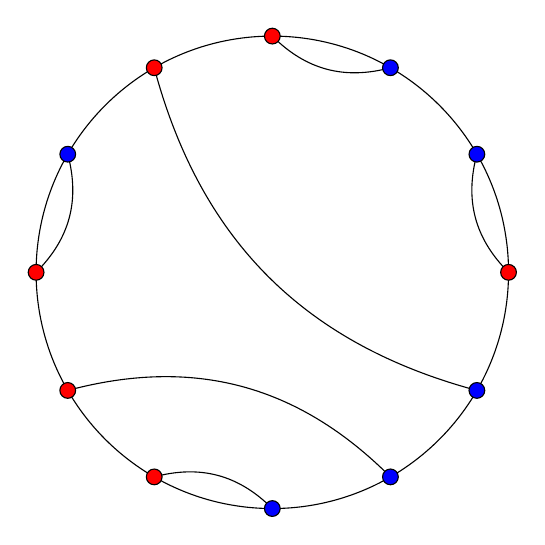
\begin{tikzpicture}
  \draw[draw] (0,0) circle (3cm);
  \draw[thin,black] (90:3) to[bend right]  (60:3);
  \draw[thin,black] (30:3) to[bend right] (0:3);
  \draw[thin,black] (120:3) to[bend right] (-30:3);
  \draw[thin,black] (180:3) to[bend right] (150:3);
  \draw[thin,black] (210:3) to[bend left] (300:3);
  \draw[thin,black] (240:3) to[bend left] (270:3);

  \draw[fill=red] (0:3) circle (0.1cm);
  \draw[fill=blue] (30:3) circle (0.1cm);
  \draw[fill=blue] (60:3) circle (0.1cm);
  \draw[fill=red] (90:3) circle (0.1cm);
  \draw[fill=red] (120:3) circle (0.1cm);
  \draw[fill=blue] (150:3) circle (0.1cm);
  \draw[fill=red] (180:3) circle (0.1cm);
  \draw[fill=red] (210:3) circle (0.1cm);
  \draw[fill=red] (240:3) circle (0.1cm);
  \draw[fill=blue] (270:3) circle (0.1cm);
  \draw[fill=blue] (300:3) circle (0.1cm);
  \draw[fill=blue] (330:3) circle (0.1cm);
\end{tikzpicture}

\vspace{0.5em}

The random process begins with the singleton set of pairs $P_1 = \inbrace{\inbrace{0,1}}$.
The process then picks one pair of unpicked elements in each iteration, till there are no more elements to pick.
Throughout the process of picking these $n/2$ pairs, it maintains the invariant that all the pairs picked till some iteration $t$, together cover exactly a contiguous arc of length $2t$ on the cycle.
Let the set of pairs picked ater iteration $t$ be $P_t$, and let the corresponding arc be $\insquare{L_t, R_t}$, with $R_t - L_t \equiv 2t (\bmod n)$.
Under the given restrictions there are three choices for the next arc to be picked, and the process picks one of these uniformly at random.
That is:
\[
  P_{t+1} =
  \begin{cases}
    P_t \cup \inbrace{\inbrace{L_t - 2, L_t - 1}} &\text{w.p. } \frac{1}{3}\\ 
    P_t \cup \inbrace{\inbrace{L_t - 1, R_t + 1}} &\text{w.p. } \frac{1}{3}\\
    P_t \cup \inbrace{\inbrace{R_t + 1, R_t + 2}} &\text{w.p. } \frac{1}{3}\\
  \end{cases}
\]
Here the additions and subtractions on the indices are \emph{modulo} $n$.
Let the final set of $n/2$ pairs be $P = P_{\frac{n}{2}}$.
The process now goes over all pairs inside $P$ and colours one variable by $\vecy$ and other by $\vecz$, uniformly at random to obtain the equipartition.

For ease of notation, we will say that both the set of $n/2$ pairs $P$ and the actual partition $\pi(P)=\vecy \sqcup \vecz$ are generated using $\mathcal{D}$.
That is, we will use both $\pi(P) \sim \mathcal{D}$ and $P \sim \mathcal{D}$.
As we mentioned earlier, the set of arc partitions is exactly the support of this distribution $\mathcal{D}$.
Similarly, an \emph{arc-full-rank} polynomial will be a polynomial $f$ for which $M_{\vecy,\vecz}(f)$ has rank $2^{n/2}$ for every arc partition $\vecy,\vecz$.\\

The task is now in two parts.
The first is to show that we can find a multilinear ABP that computes an \emph{arc-full-rank} polynomial $f$.
Then, we have to show that any small multilinear formula is rank-deficient under a random arc-partition.

\section{Upper bound with ABPs}

We want the hard polynomial to have full rank with respect to every arc partition, so let us see how we can come up with a full rank polynomial for a fixed partition $\vecy \sqcup \vecz$.
Say $\vecy = \inbrace{y_1,\ldots,y_m}$ and $\vecz = \inbrace{z_1,\ldots,z_m}$.
We know that the polynomial $P(\vecy,\vecz) = \Pi_{i \in [m]} (y_i + z_i)$ has full rank with respect to the given partition.

Now we want to extend this idea to having full rank over any arc partition.
One way to do this is to add a few (at most polynomially many) extra variables $\vecw$ so that for any arc partition $\pi$ there will be an assignment $\phi$ to $\vecw$ that will ensure that $F_n(\phi(\vecw),\pi(\vecx))$ looks like $P(\vecy,\vecz)$.
We are going to do just that and additionally ensure that $F_n$ is still computable by a small multilinear ABP.

Recall that for sampling of pairs from $\mathcal{D}$ we maintained the invariant that the pairs in $P_t$ cover a contiguous arc $\insquare{L_t, R_t}$ of length exactly $2t$ on the $n$-cycle.
This gives us that for any $t$, after $t$ steps the number of distinct $P_t$s possible, is at most $n$.
Moreover for the $(t+1)^{th}$ sampling step it is enough just to know $L_t$ and $R_t$.
This helps us construct the following ABP of width $\leq n$ and $n/2$ layers, that we describe by describing the underlying graph.\\

Let the nodes in each layer $t$ be labelled as $v_1^{(t)},\cdots, v_n^{(t)}$.
The node $v_i^{(t)}$ would correspond to the fact that the current arc is $[i,i+2t] \bmod{n}$.
We now describe the edges of the ABP.
There would be three edges out of $v_i^{(t)}$ and they are as follows:

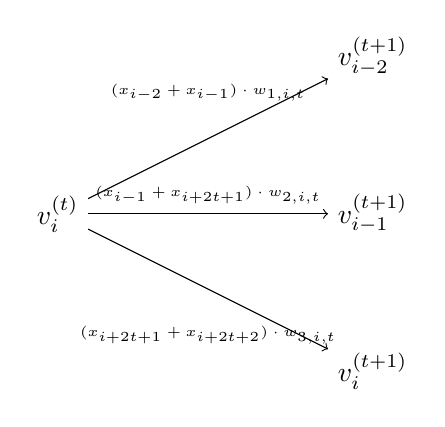
\begin{tikzpicture}
  \node (vj) at (0,0) {$v_i^{(t)}$};
  \node (v1) at (4,2) {$v_{i-2}^{(t+1)}$}
  edge[<-] node [midway,above=10pt] {{\tiny $(x_{i-2} + x_{i-1})\cdot w_{1,i,t}$}} (vj);
  \node (v2) at (4,0) {$v_{i-1}^{(t+1)}$}
  edge[<-] node [midway,above] {{\tiny $(x_{i-1} + x_{i+2t+1})\cdot w_{2,i,t}$}} (vj);

  \node (v3) at (4,-2) {$v_{i}^{(t+1)}$}
  edge[<-] node [midway,below=10pt] {{\tiny $(x_{i+2t+1} + x_{i+2t+2})\cdot w_{3,i,t}$}} (vj);
\end{tikzpicture}

The ABP therefore has $O(n^2)$ vertices and since there are three edges out of each vertex, there are $O(n^2)$ edges.
The polynomial computed by the ABP, $F_n$, would be our hard polynomial.
From the construction, the following lemma is easy to verify and is left as an easy exercise.

\begin{exercise}
  Show that the polynomial $F_n$ constructed above is full-rank with respect to every arc-partition.
\end{exercise}


\subsection{Lower bound against formulas}

As seen earlier in \autoref{chap:multilinear}, we will prove the lower bound by proving that the probability of a \emph{log-product term} having rank that is $n^{\delta}$ close to full is inverse quasipolynomially small (for some small enough $\delta > 0$).
The difference here is the distribution is over the arc-partitions and not the uniform distribution.

Suppose $|X| = n$.
As in the previous settings, we have a partition $X = X_1 \sqcup \cdots \sqcup X_t$ from our log-product decomposition with $k = \Theta(\log n)$ and $\abs{X_i} \geq |X|^{7/8}$ for all $i$.
We'll refer to each $X_i$ as a bucket.
If we pick an arc-partition at random, we would like to estimate the probability that none of the $X_i$'s are $n^\delta$ unbalanced.
We would like to show that this is inverse quasi-polynomially small.

Arc partitions are chosen by first choosing a pairing $P$ and then bi-colouring each pair $p \in P$.
Firstly, note that if $X_i$ picks up only ``whole pairs'' from the set of pairs $P$, then no matter how we bi-colour each pair we would have $X_i$ being completely balanced.
It is therefore sensible to look at buckets that pick up exactly one element from a lot of pairs.
\begin{align*}
	 V_i(P) &= \setdef{ p \in P}{\abs{ p \cap X_i } = 1 }\\
	G(P) &= \setdef{ i \in [t]}{\abs{ V_i(P) } \geq n^{1/1000} }
\end{align*}

The set $G(P)$ refers to the ``good buckets'' that \emph{cut} many pairs; the colours of these end-points are completely independent.
Therefore, at the very least, for each $i \in G(P)$, we can hope to say that the probability that $X_i$ is not $n^{\delta}$-unbalanced is small (inverse polynomial).

\begin{lemma}
  \label{lem:MLSep:bound-for-good-buckets}
  Let $P$ be a partition of $X$ into pairs and let $G(P)$ be as defined above. 
  Then, for any $i \in G(P)$,
  \[
    \Pr[ \text{$X_i$ is $n^{\delta}$-balanced} ] \leq O\pfrac{2n^{\delta}}{n^{1/2000}}
  \]
  where the probability is over a random bi-colouring of the pairs in $P$. 
\end{lemma}

This lemma is easy to prove.
If the set $G(P)$ is large, we can then hope to say that we have a good number of independent events and hope for an inverse quasi-polynomial probability.

\subsubsection*{Arranging for many independent events}

The following lemma states that for most pairings $P \sim \mathcal{D}$ we must have many buckets in $G(P)$.
This is the most technical part of the paper and we'll see a very rough sketch in the next section.

\begin{lemma}
\label{lem:manyBucketsWithCuts}
Given a partition $X = X_1 \sqcup \cdots \sqcup X_t$ with $t = \Theta(\log n)$ and $\abs{X_i} \geq n^{7/8}$ for all $i \in [t]$. Then,
\[
 \Pr_{P \in \mathcal{D}} \insquare{ \abs{G(P)} \leq \frac{t}{1000} } \leq n^{- \Omega(t)}
\]
where $\mathcal{D}$ is the distribution for arc partitions.
\end{lemma}

Hence, with high probability we have $|G(P)| \geq t/1000 = \Theta(\log n)$.
Now we would like to say that there are many (almost) independent events among these good buckets.

Assume the good buckets are $X_1,\ldots,X_{r}$ without loss of generality.
From \autoref{lem:MLSep:bound-for-good-buckets}, we know that the probability that $X_1$ is too balanced is small.
However we now want to argue the same for $X_2$, even after we condition on $X_1$ being too balanced.
This need not always be true.
Consider the setting that both $X_1 \union X_2$ is a just a union of pairs, but each pair has one end-point in $X_1$ and the other in $X_2$.
Now if $X_1$ is very balanced, then $X_2$ would also be very balanced.

Thus, in order to say $X_2$ would likely be unbalanced even after conditioning on $X_1$ being balanced, we need to say that $X_2$ has many \emph{other} pairs that are cut (that is, these aren't accounted for in $X_1$).
More generally, want to ensure that for each $i \in [r]$, the bucket $X_i$ cuts many pairs $p \in P$ whose other end-point is \emph{not} in $X_1 \sqcup \cdots \sqcup X_{i-1}$.\\

Let us consider a graph $H(P)$ with the buckets $[t]$ as vertices and let us mark the good buckets $[r]$ as red.
Add an edge $(i,j)$ if $\abs{V_i(P) \cap V_j(P)} \geq n^{1/1500}$; that is there are many pairs with one end-point in $i$ and one in $j$.
Note that each good bucket $i$ has degree at least $1$ in $H(P)$ as each good bucket cuts $n^{1/1000}$ pairs and we only have $O(\log n)$ buckets.

\begin{lemma}
\label{lem:halfVerticesIndep}
There exists a sequence $B=\inparen{b_1,\ldots,b_\ell}$ of good buckets from $H(P)$ with  $\ell \geq \frac{r}{2}$ such that for all $i \in [\ell]$, the vertex $b_i$ in the graph $H(P) \setminus \set{b_1,\ldots, b_{i-1}}$ has degree $\geq 1$.
\end{lemma}
\begin{proof}
  Consider a spanning forest of $H(P)$.
Since every good bucket has degree at least $1$, the spanning forest has at least $r/2$ edges emanating from good buckets.
The required sequence of vertices can be obtained by repeatedly removing leaves of this forest.
\end{proof}

Let $(b_1,\ldots,b_\ell)$ be such a sequence for $H(P)$, with $\ell \geq r/2 = \Omega(t)$.
For brevity, let pairs that are not cut by any of the $b_i$s be $\tilde{P}$.
For every $i \in [r]$, define by $P_i$ the pairs from $\inparen{ P \setminus \inparen{ P_1 \cup \cdots \cup P_{i-1}} }$ that are cut by $b_i$.
Now view the random colouring $\pi(P)$ of pairs from $P$ to be happening in the order $P_1,\ldots,P_r,\tilde{P}$.
From \autoref{lem:halfVerticesIndep} we have that $\abs{P_i} \geq n^{1/1500}$ for all $i \in [r]$.
As mentioned above, this will help us yield an inverse polynomial factor for each of the $r$ buckets, even after conditioning on previous colourings.
Also let $n_i = \abs{b_i}$ and for $\pi(P)=\vecy,\vecz \sim \mathcal{D}$, let $y_i = \abs{b_i \cap \vecy}$.
Let $\delta > 0$ be a suitably small constant.
For $i \in [r]$, let the $E_i$ refer to the event that $\abs{y_i - n_i/2} \leq n^{\delta}$.
In the case when $\abs{G(P)} \geq K/1000$, we get that
\begin{align*}
\Pr_{\pi(P)=\vecy,\vecz \sim \mathcal{D}} \insquare{\operatorname{rank}\inparen{M_{Y,Z}(g)} \geq 2^{n/2 - n^{\delta}}} &\leq \Pr_{\pi(P)=\vecy,\vecz \sim \mathcal{D}} \insquare{\bigwedge_{i \in [r]} E_i}\\
&= \prod_{i \in [r]} \Pr_{\pi(P)=\vecy,\vecz \sim \mathcal{D}} \insquare{E_i \Big{|} \bigwedge_{j < i} E_j }\\
&\leq \prod_{i \in [r]} O\inparen{\frac{2n^{\delta}}{\sqrt{\abs{P_i}}}}\\
&\leq \prod_{i \in [r]} n^{-\Omega(1)} = n^{-\Omega(K)}.
\end{align*}

\noindent
Combining this with the fact that $G(P)$ must be large with high probability (\autoref{lem:manyBucketsWithCuts}), we get
\begin{align*}
&\Pr_{\pi(P)=\vecy,\vecz \sim \mathcal{D}} \insquare{\operatorname{rank}\inparen{M_{Y,Z}(g)} \geq 2^{n/2 - n^{\delta}}} &\\
&\leq \Pr_{\pi(P)=\vecy,\vecz \sim \mathcal{D}} \insquare{\operatorname{rank}\inparen{M_{Y,Z}(g)} \geq 2^{n/2 - n^{\delta}} \Big{|} \abs{G(P)} \geq K/1000} \Pr_{P \sim \mathcal{D}} \insquare{\abs{G(P)} \geq K/1000}\\
&  \qquad \quad+ \Pr_{P \sim \mathcal{D}} \insquare{\abs{G(P)} \leq K/1000}\\
&\leq n^{-\Omega(K)}+ n^{-\Omega(K)} = n^{-\Omega(\log n)}. 
\end{align*}
This would finally complete the proof of \autoref{thm:separation}.

\section{Proof sketch for Lemma \ref{lem:manyBucketsWithCuts}}

We will a brief sketch of the proof of \autoref{lem:manyBucketsWithCuts}.
The full proof is quite invovled and a full description can of course be found in their paper \cite{dmpy12}.
We will try to give a rough sketch of the main ideas in the proof. \\

We will call an index $j$ a \emph{jump} with respect to the bucket $X_k$, if $x_j \in X_k$ and $x_{j+1} \notin X_k$.
The following observation is easy to see.

%%%%%%%%%%%%%%%%%%%%%%%%%%%%%%%%%%%%%%%%%%%%%%%%%%%

\begin{observation}\label{obs:jumps-cut}
  For any $j\neq 0,1$, the probability that $(j,j+1)$ is chosen as a pair by an arc partition is at least $1/9$. 
\end{observation}

Therefore, if we have many buckets with lots of jumps, then a lot of them would contribute pairs that are cut.
More formally, suppose we have more then $K/2$ buckets with at least $N = n^{1/100}$ jumps.
We then collect at most $N$ jumps from each bucket to get a total of $\geq KN/2$ distinct indices.
\autoref{obs:jumps-cut} says the probability that a particular jump results in a pair that is cut bounded below by some constant.
We therefore conclude that $\geq KN/100$ of the total jumps get converted into cuts with high probability.
Since we chose at most $N$ jumps from each bucket, this means that at least $K/1000$ buckets contribute at least $N^{1/10} = n^{1/1000}$ cuts, which proves \autoref{lem:manyBucketsWithCuts} for this case.

\medskip

The trickier case is when there aren't many buckets with a lot of jumps.
Let us consider an extreme case to understand this better --- buckets form large contiguous segments of the circle.

Suppose we have a partial arc $[L_t,R_t]$, and suppose we have two different buckets $X_i$ and $X_j$ on the two ends that are to be processed.
If these segments are sufficiently large, then a constant fraction of these would be matched between $X_i$ and $X_j$ (via the $(L_t-1,R_t+1)$ sort of pairs) with high probability, making both $i$ and $j$ good buckets.

The other case could be that the two segments at the ends of $L_t$ and $R_t$ belong to the same bucket say $X_i$.
Let us call these segments $A_L$ and $A_R$ and let their lengths be $a_L$ and $a_R$.
The next few pairs would not yield any cuts as they will below to the same bucket.
But the key insight is this --- consider the arc partition when one of the two sides is completely processed (that is, $A_L$ or $A_R$ is completely contained in $[L_{t'},R_{t'}]$ at that time).
When this happens, the probability that there are very few elements left in the other part is inverse polynomially small.
This is once again very similar to the fact that a random partition would not cut a set in too balanced a fashion.
In similar spirit, the probability that there are too few elements in $A_L$ left after $A_R$ has been completely processed (or vice-versa) is inverse polynomially small.
Hence, we would essentially reduce to the previous case when we have two sufficiently large segments from different buckets on the ends of $L_t$ and $R_t$.
Therefore, the probability that $i$ fails to be a part of $G(P)$ is inverse polynomially small, and these events are almost independent for various $i$'s.
Therefore, the probability that $G(P) < t/1000$ is at most $n^{-\Omega(t)}$ as claimed by \autoref{lem:manyBucketsWithCuts}.


The formal proof requires some careful analysis and Dvir~et~al.~\cite{dmpy12} do this by considering the process as a ``random walk on a distorted chess board''. 

\section{What about $\IMM$?}

The result of Dvir, Malod, Perifel and Yehudayoff \cite{dmpy12} that we dicussed separate the classes of syntactic multilinear ABPs and multilinear formulas.
A natural question is whether this also works for the iterated matrix multiplication polynomial ($\IMM$).
Note that the polynomial used for this lower bound was a syntactic multilinear ABP but is \emph{not} a multilinear projection of $\IMM$!
The same variable may occur in many edges even though each path may use each variable at most once.
Therefore, such a reduction does not follow from this proof.
In fact, this is an important open problem.

\begin{openproblem}[Multilinear formula lower bounds for $\IMM$]
  Show that $\IMM_{n,d}$ requires  multilinear formulas of $(nd)^{\Omega(\log nd)}$ to compute it. 
\end{openproblem}


%%% Local Variables:
%%% mode: latex
%%% TeX-source-correlate-method-active: synctex
%%% TeX-master: "fancymain"
%%% End:
